\documentclass{article}


% if you need to pass options to natbib, use, e.g.:
%     \PassOptionsToPackage{numbers, compress}{natbib}
% before loading neurips_2025

\PassOptionsToPackage{numbers, sort, compress}{natbib}

% ready for submission
\usepackage{neurips_2025}


%\bibliographystyle{abbrvnat}
\bibliographystyle{unsrtnat}


\usepackage[pdftex]{graphicx}
\usepackage{amsmath}
% to compile a preprint version, e.g., for submission to arXiv, add add the
% [preprint] option:
%\usepackage[preprint]{neurips_2025}


% to compile a camera-ready version, add the [final] option, e.g.:
%     \usepackage[final]{neurips_2025}


% to avoid loading the natbib package, add option nonatbib:
%    \usepackage[nonatbib]{neurips_2025}


\usepackage[utf8]{inputenc} % allow utf-8 input
\usepackage[T1]{fontenc}    % use 8-bit T1 fonts
\usepackage{hyperref}       % hyperlinks
\usepackage{url}            % simple URL typesetting
\usepackage{booktabs}       % professional-quality tables
\usepackage{amsfonts}       % blackboard math symbols
\usepackage{nicefrac}       % compact symbols for 1/2, etc.
\usepackage{microtype}      % microtypography
\usepackage{xcolor}         % colors

\newcommand\reynotes[1]{\textcolor{purple}{#1}}

%\title{SmokeViz: Using Pseudo-Labels to Develop a Human-Labeled Deep Learning Dataset of Wildfire Smoke Plumes in Satellite Imagery}
\title{SmokeViz: A Large-Scale Satellite Dataset for Wildfire Smoke Detection and Segmentation}


% The \author macro works with any number of authors. There are two commands
% used to separate the names and addresses of multiple authors: \And and \AND.
%
% Using \And between authors leaves it to LaTeX to determine where to break the
% lines. Using \AND forces a line break at that point. So, if LaTeX puts 3 of 4
% authors names on the first line, and the last on the second line, try using
% \AND instead of \And before the third author name.


\author{%
  Rey Koki\\%\thanks{rey.koki@colorado.edu} \\
  Department of Computer Science\\
  University of Colorado Boulder\\
  Boulder, Colorado 80303\\
  \texttt{rey.koki@colorado.edu} \\
  % examples of more authors
  % \And
  % Coauthor \\
  % Affiliation \\
  % Address \\
  % \texttt{email} \\
  % \AND
  % Coauthor \\
  % Affiliation \\
  % Address \\
  % \texttt{email} \\
  % \And
  % Coauthor \\
  % Affiliation \\
  % Address \\
  % \texttt{email} \\
  % \And
  % Coauthor \\
  % Affiliation \\
  % Address \\
  % \texttt{email} \\
}


\begin{document}






\appendix

\section{Supplementary Material}

\section{A. Original Data and Software Licenses}

The HMS smoke product does not have a license attached to it. For GOES imagery, NOAA states: \emph{"There are no restrictions on the use of this data"}. PyTroll is distributed under the GNU General Public License v3.0, and Segmentation Models PyTorch is distributed under the MIT License.

\section{B. Satellite and Band Selection}


As described in the main paper, Advanced Baseline Imager (ABI) bands 1-3 were selected for their high signal-to-noise ratio (SNR) and relevance to visible smoke. Figure \ref{G16_vs_G17} shows an example of GOES-West provides higher visibility of a smoke plume than GOES-East near sunrise. This effect is consistent with Mie scattering physics, where forward-scattered light enhances contrast for aerosols like smoke under favorable solar geometry.

\setcounter{figure}{9}

\begin{figure}[!htb]
    \centering
    \includegraphics[width=\linewidth]{figures/G17_s20221371250321_35.61_-105.01_36.png}
    \caption{(a) True color GOES-EAST (top) and GOES-WEST (bottom) imagery from May \(18^{th}\), 2022 centered at (\(35.6^{\circ}\), \(-105.0^{\circ}\)) in New Mexico, USA taken at 12:50 UTC. The GOES-East and West raw band imagery for (c) blue, (d) red and (e) veggie bands show variations in the SNR for smoke detection in relation to the \(\lambda\) of light being measured.}\label{G16_vs_G17}
\end{figure}

Figure \ref{all_bands} presents a smoke plume in a cloudy scene across all 16 ABI bands described in Table \ref{band_table}. The smoke signal is prominent in Bands 1–3 but diminishes in subsequent NIR channels. Band C07 (3.9 \(\mu\)m), which is sensitive to thermal anomalies, shows a strong fire signal at the source of the plume. While useful for active fire detection, including C07 for smoke segmentation may bias models toward learning fire-smoke co-location, reducing generalization to detached or low opacity smoke plumes, especially those classified as light density that have traveled far from the source. This concern supports the decision to limit input channels in SmokeViz to those that reflect the analyst operational view while minimizing potential modeling shortcuts and dataset size. The SmokeViz dataset development code is designed to be easily adapted to incorporate any desired spectral bands and/or composites.


\begin{figure}[!htb]
    \centering
    \includegraphics[width=\linewidth]{figures/G16_s20221550056176_33_-106_all_band.png}
    \caption{GOES-EAST imagery for all 16 bands from June \(5^{th}\), 2022 centered at (\(33.0^{\circ}\), \(-106.0^{\circ}\)) in New Mexico, USA taken at 00:56 UTC.}\label{all_bands}
\end{figure}

\begin{table}[!htb]
\centering
\caption{The GOES-Series Advanced Baseline Imager (ABI) provides data at 16 channels that cover visible (C01-C02), near-IR (C03-C06) and IR (C07-C16) bands.}
\begin{tabular}{llcc}
\toprule
\textbf{Band} & \textbf{Description} & \textbf{Center Wavelength (\(\mu\)m)} & \textbf{Spatial Resolution (km)} \\
\midrule
C01  & Blue visible                & 0.47     & 1   \\
C02  & Red visible                 & 0.64     & 0.5 \\
C03  & Veggie near IR             & 0.865    & 1   \\
C04  & Cirrus                     & 1.378    & 2   \\
C05  & Snow/Ice                   & 1.61     & 1   \\
C06  & Cloud particle             & 2.24     & 2   \\
C07  & Shortwave IR               & 3.9      & 2   \\
C08  & Upper-level water vapor    & 6.2      & 2   \\
C09  & Mid-level water vapor      & 6.9      & 2   \\
C10  & Lower-level water vapor    & 7.3      & 2   \\
C11  & IR cloud phase             & 8.5      & 2   \\
C12  & Ozone                      & 9.6      & 2   \\
C13  & Clean longwave IR          & 10.35    & 2   \\
C14  & Longwave IR                & 11.2     & 2   \\
C15  & Dirty longwave IR          & 12.3     & 2   \\
C16  & CO\(_2\)                         & 13.3     & 2   \\
\bottomrule
\end{tabular}
\label{band_table}
\end{table}

\subsection{Statistical Dataset Visualizations}

Figures \ref{num_frames}-\ref{count_per_country} summarize key statistical characteristics of the SmokeViz dataset.

Figure \ref{num_frames} presents a histogram of the number of GOES satellite frames associated with each HMS annotation. Since frames are available every 10 minutes, this visualization reflects the variability in annotation time window duration. Most annotations span between 5 and 50 frames, corresponding to 50 minutes to just over 8 hours, underscoring the need for resolving temporal ambiguity during dataset refinement.

Figure \ref{count_per_yr} shows the number of SmokeViz samples per year, stratified by smoke density. The year 2020 exhibits the highest sample count, aligning with an exceptionally active wildfire season across North America \cite{fires2020}. The density distribution across years also varies, with some years showing a higher relative proportion of light or medium smoke annotations.

Lastly, SmokeViz includes annotations across North America, Figure \ref{count_per_country} summarizes the dataset's geographic coverage by country, including the United States, Canada, and Mexico.



\begin{figure}[!htb]
    \centering
        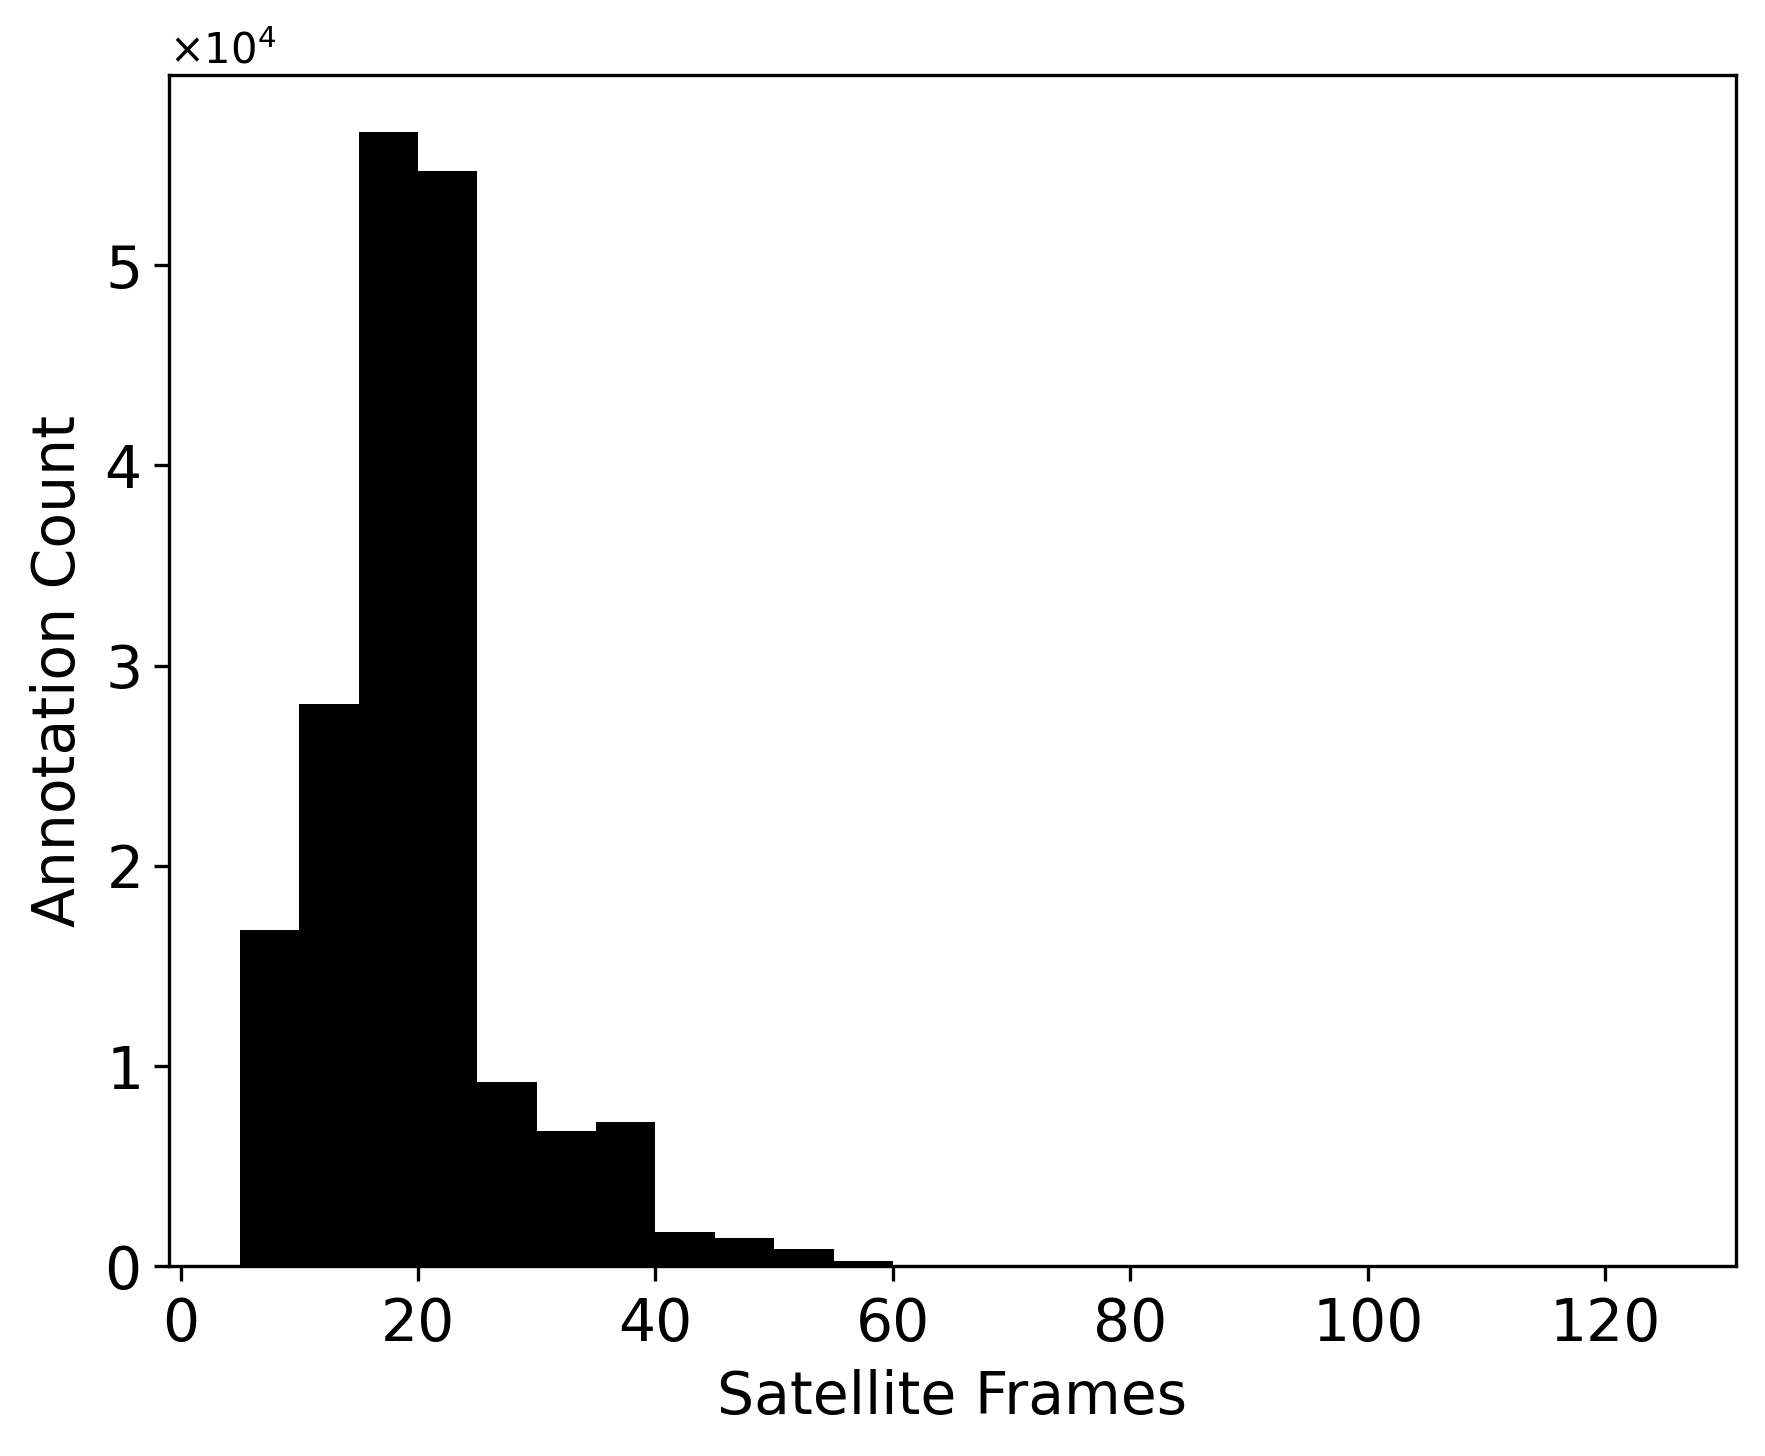
\includegraphics[width=0.49\textwidth]{stat_figs/sample_count_vs_frames.png}
        \caption{The number of annotations that span a number of satellite frames that are generated at a 10-minute interval.}
        \label{num_frames}
\end{figure}

\begin{figure}[!htb]
    \parbox{\textwidth}{
      \parbox{0.49\textwidth}{
        \centering
        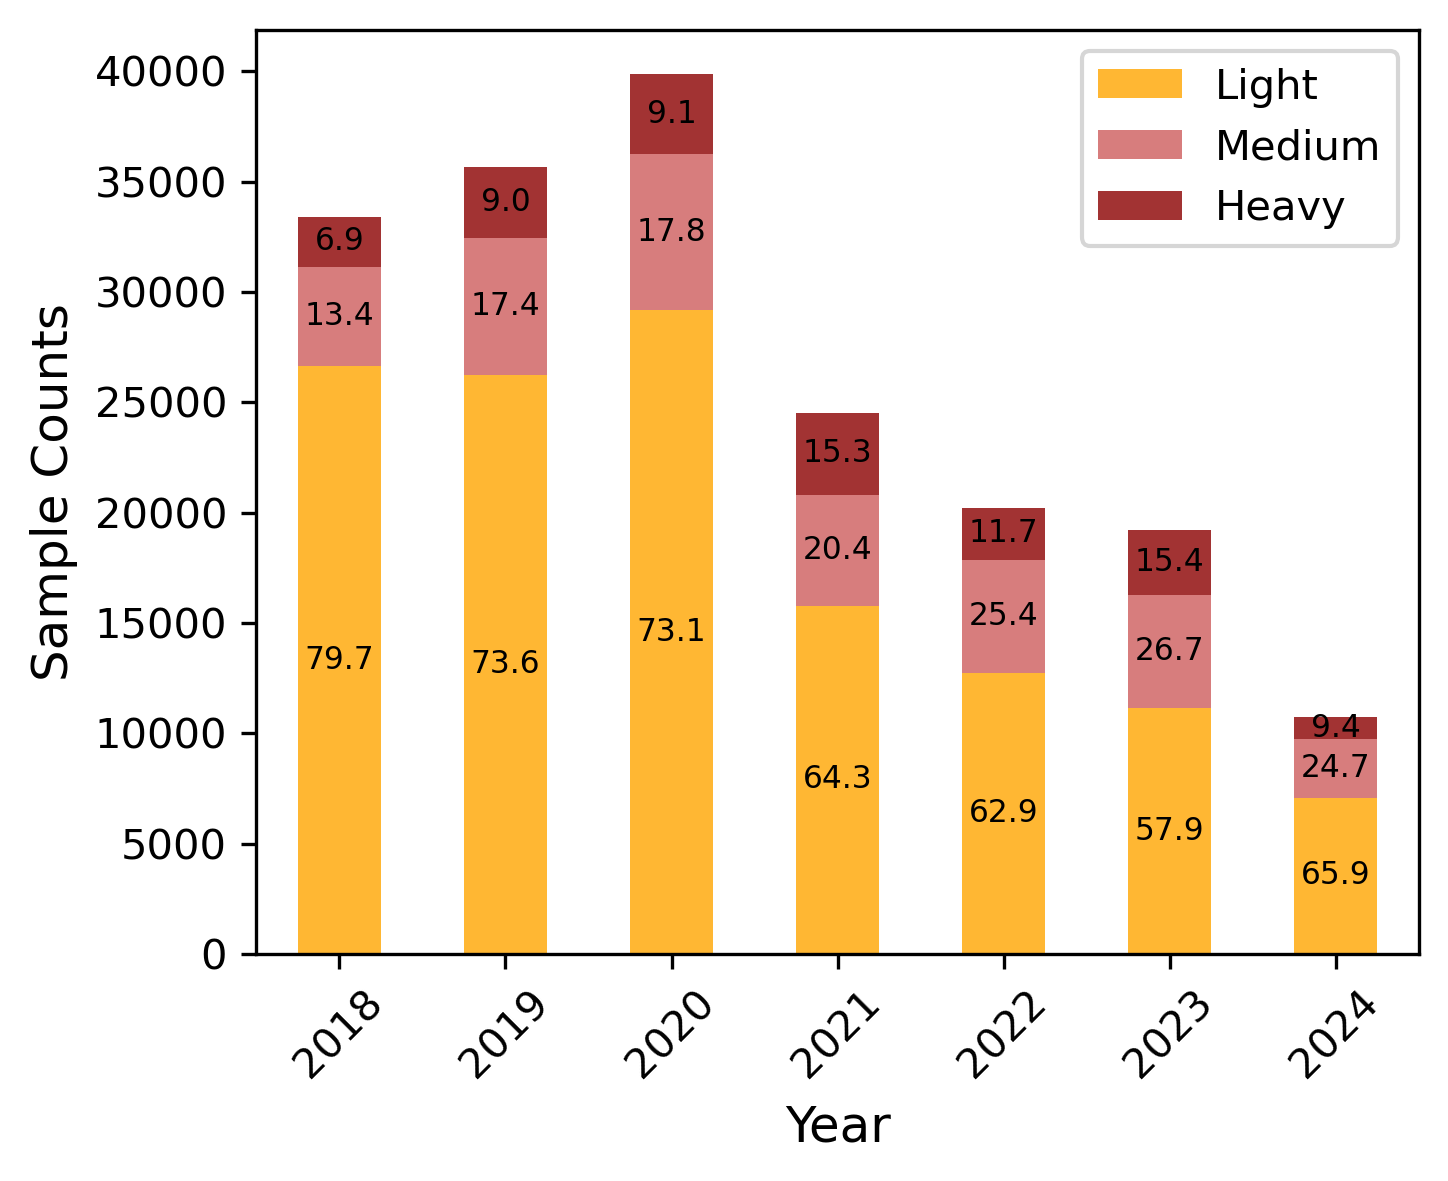
\includegraphics[width=0.49\textwidth]{stat_figs/sample_count_per_yr_percentages.png}
        \caption{Annual sample counts in the SmokeViz dataset, broken down by smoke density class. Percentages within each column indicate the relative frequency of each density level for that year.}
        \label{count_per_yr}
      }
    \hspace{0.01\textwidth}
      \parbox{0.49\textwidth}{
        \centering
        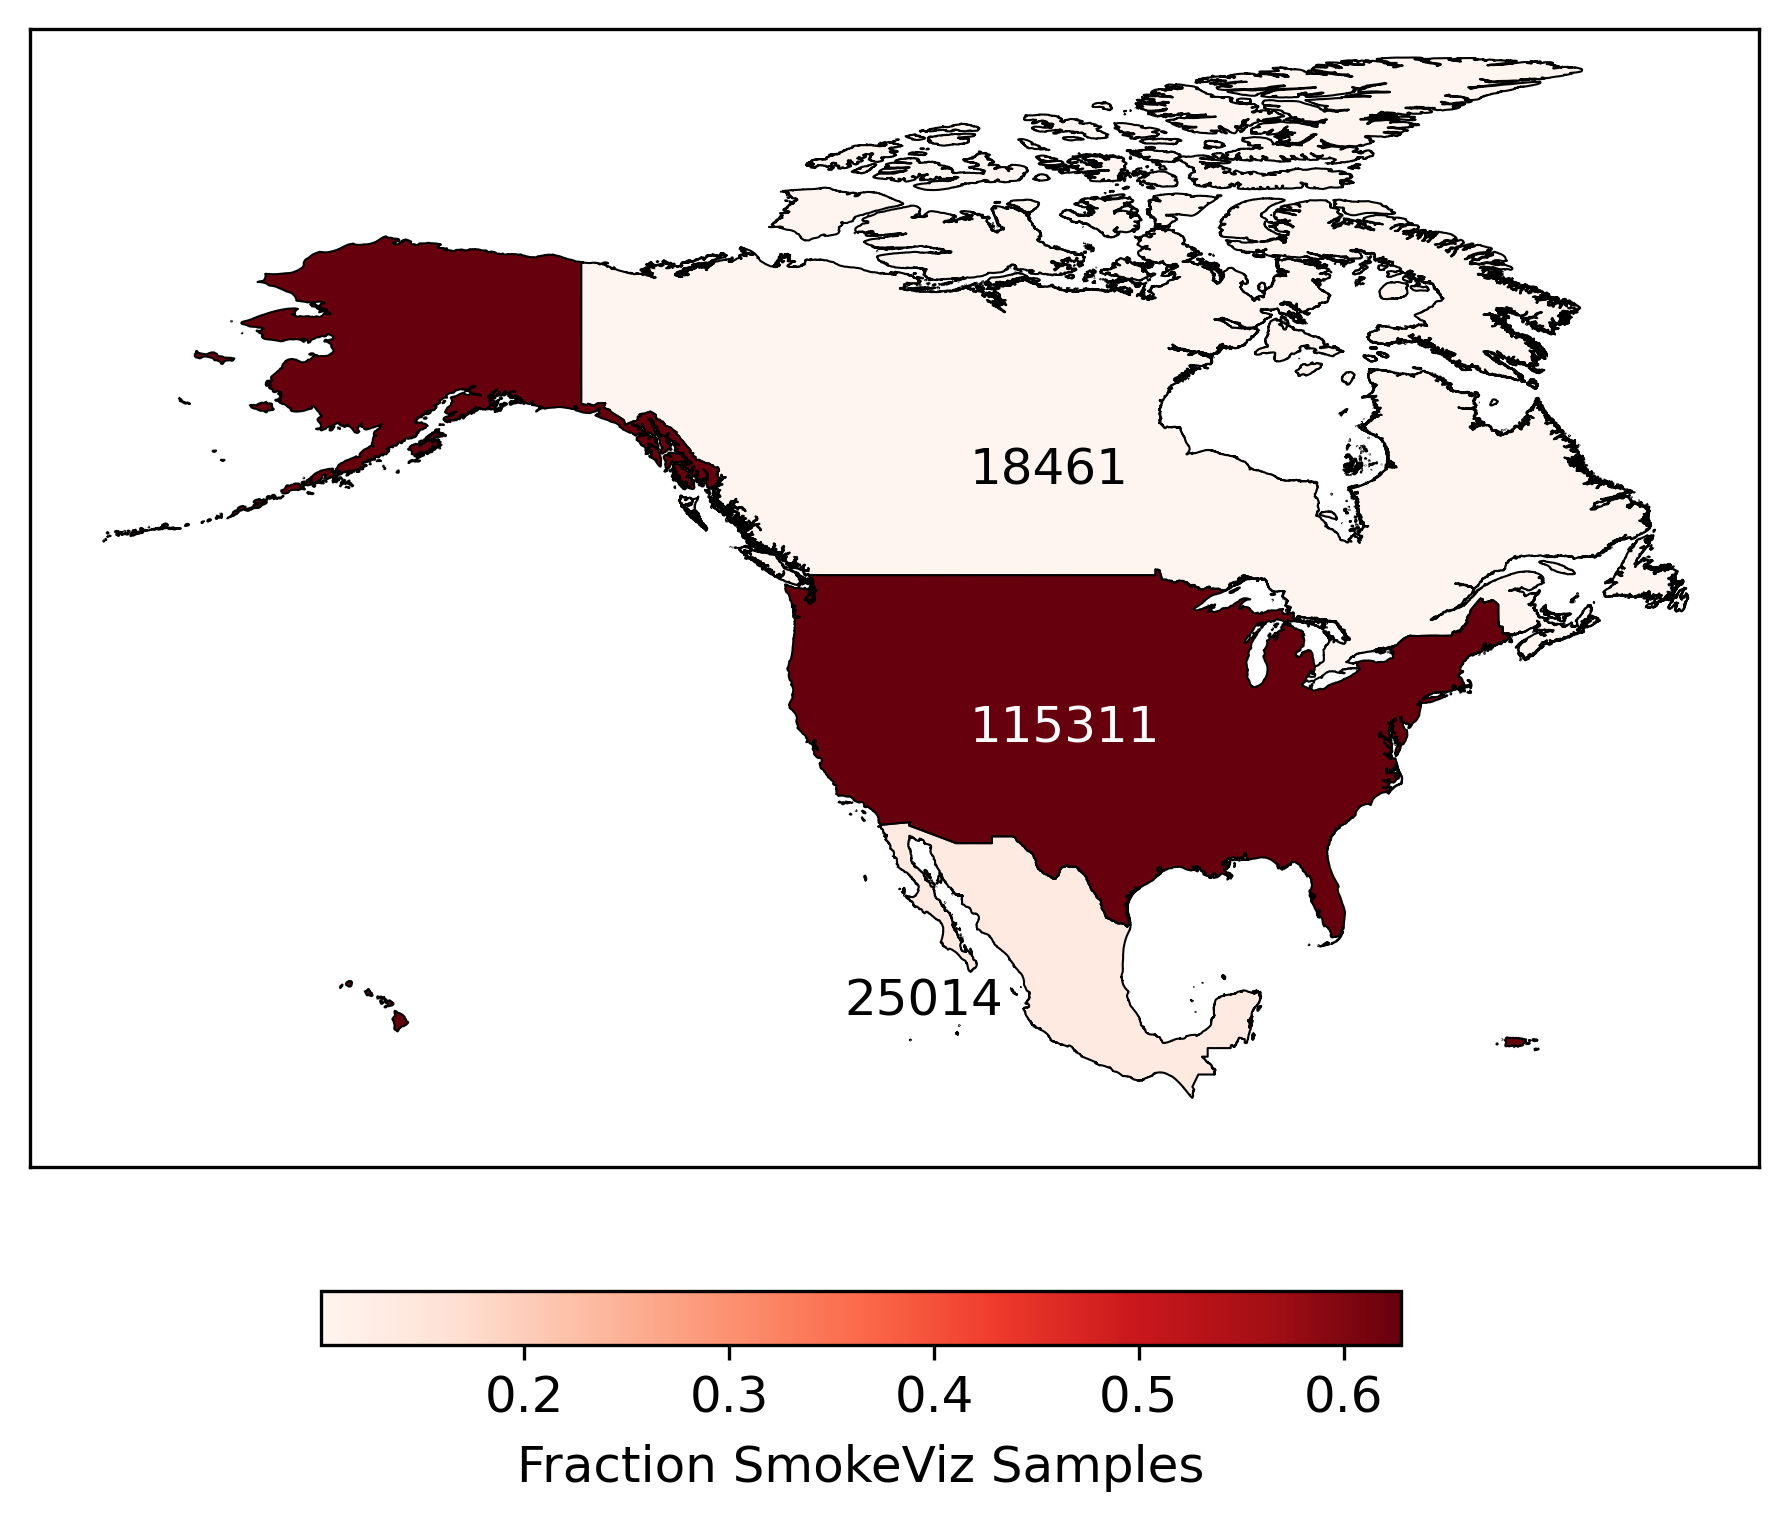
\includegraphics[width=0.49\textwidth]{stat_figs/sample_percent_country.png}
        \caption{Proportion of samples in the SmokeViz dataset whose center pixel falls within Canada, the U.S.A., or Mexico. Sample counts are: Canada: 18,461; U.S.: 115,311; Mexico: 25,014. An additional 24,886 samples are centered over other countries or oceans.}
        \label{count_per_country}
      }
    }
\end{figure}

\subsection{Agricultural Burns}

The monthly peak in sample counts, discussed in the main text (Figure 6), appears in March and April, prior to the typical wildfire season that spans late spring through fall. This early peak is likely driven by prescribed agricultural burns, which are commonly conducted before vegetation exits winter dormancy \cite{ag_fire}. Figure 6 from the main text also shows variations in overall IoU values running \(f_{c}\) on the \(\mathcal{D}_p\) test set data per month. The highest IoU values are during the typical wildfire season and outside the typical window for prescribed agricultural burns. In addition, Figure 7 from the main text shows that the highest sample counts occur in California, Georgia, and Florida. The elevated number of annotations in southeastern states may be explained by the prevalence of agricultural burns in that region. Since HMS annotations do not differentiate between prescribed burns and wildfires, the dataset includes both event types. Users interested in isolating wildfire events may consider filtering out short-duration annotations (e.g., those lasting only a single day), though this may be complicated by variability in analyst-defined time windows and annotation frequency per fire.

In order to observe geographical regional variations we create quadrants, Northwest (NW), Southwest (SW), Northeast (NE) and Southeast (SE) in relation to the midpoint (40, -105) and show the sample distribution and model performance for each region in table \ref{quad}. The table shows the worst \(f_c\) performance in the SE quadrant despite representing this largest fraction of the training data. This is likely due to the large number of aforementioned prescribed burns in that area. If the goal of the dataset is to be used to train a model to detect and monitor large wildfires, a weakness in the dataset would be that it likely consists of a lot more small, controlled agricultural burns that aren't representative of the intended task. 

\begin{table}
    \caption{Along with sample count we show variations in \(f_{c}\) performance depending on quadrant.}
  \label{quad}
  \centering
  \begin{tabular}{llll}
    \toprule
    Quadrant & \(\mathcal{D}_p\) Test IoU & \(\mathcal{D}_p\) Test Samples & \(\mathcal{D}_p\) Samples \\
    \midrule
    NW & 0.5887 & 4177 & 32792\\
    SW & 0.4590 & 1937 & 34267\\
    NE & 0.5822 & 1133   & 13342\\
    SE & 0.4798 & 12977 & 103271 \\
    \bottomrule
  \end{tabular}
\end{table}




\subsection{Satellite Analysis}


We report on how many samples come from each satellite in Figure \ref{sat_dataset}, along with the \(\mathcal{D}_p\) test set IoU. While GOES-EAST provides over triple the number of training samples, \(f_c\) performs better on GOES-WEST samples out of the test set. The signal observed by a single satellite vary diurnally and annually in the amount of atmospheric noise and solar radiation. In turn, if provided with enough samples, this could create a more robust and generalizable model to the extent of being able to perform well on two different sensors with varying calibrations and line of sights. Note that on June 18, 2022, GOES-West switch from operational satellite GOES-17 to the new satellelite GOES-18 satellite. The overall IoU from GOES-17 to GOES-18 is 0.6262 to 0.5852. Training data from 2018-2021 used GOES-17 only training data from 2024 includes GOES-18, so it makes sense that GOES-18 would perform worse than GOES-17. 

\begin{figure}[!htb]
    \centering
    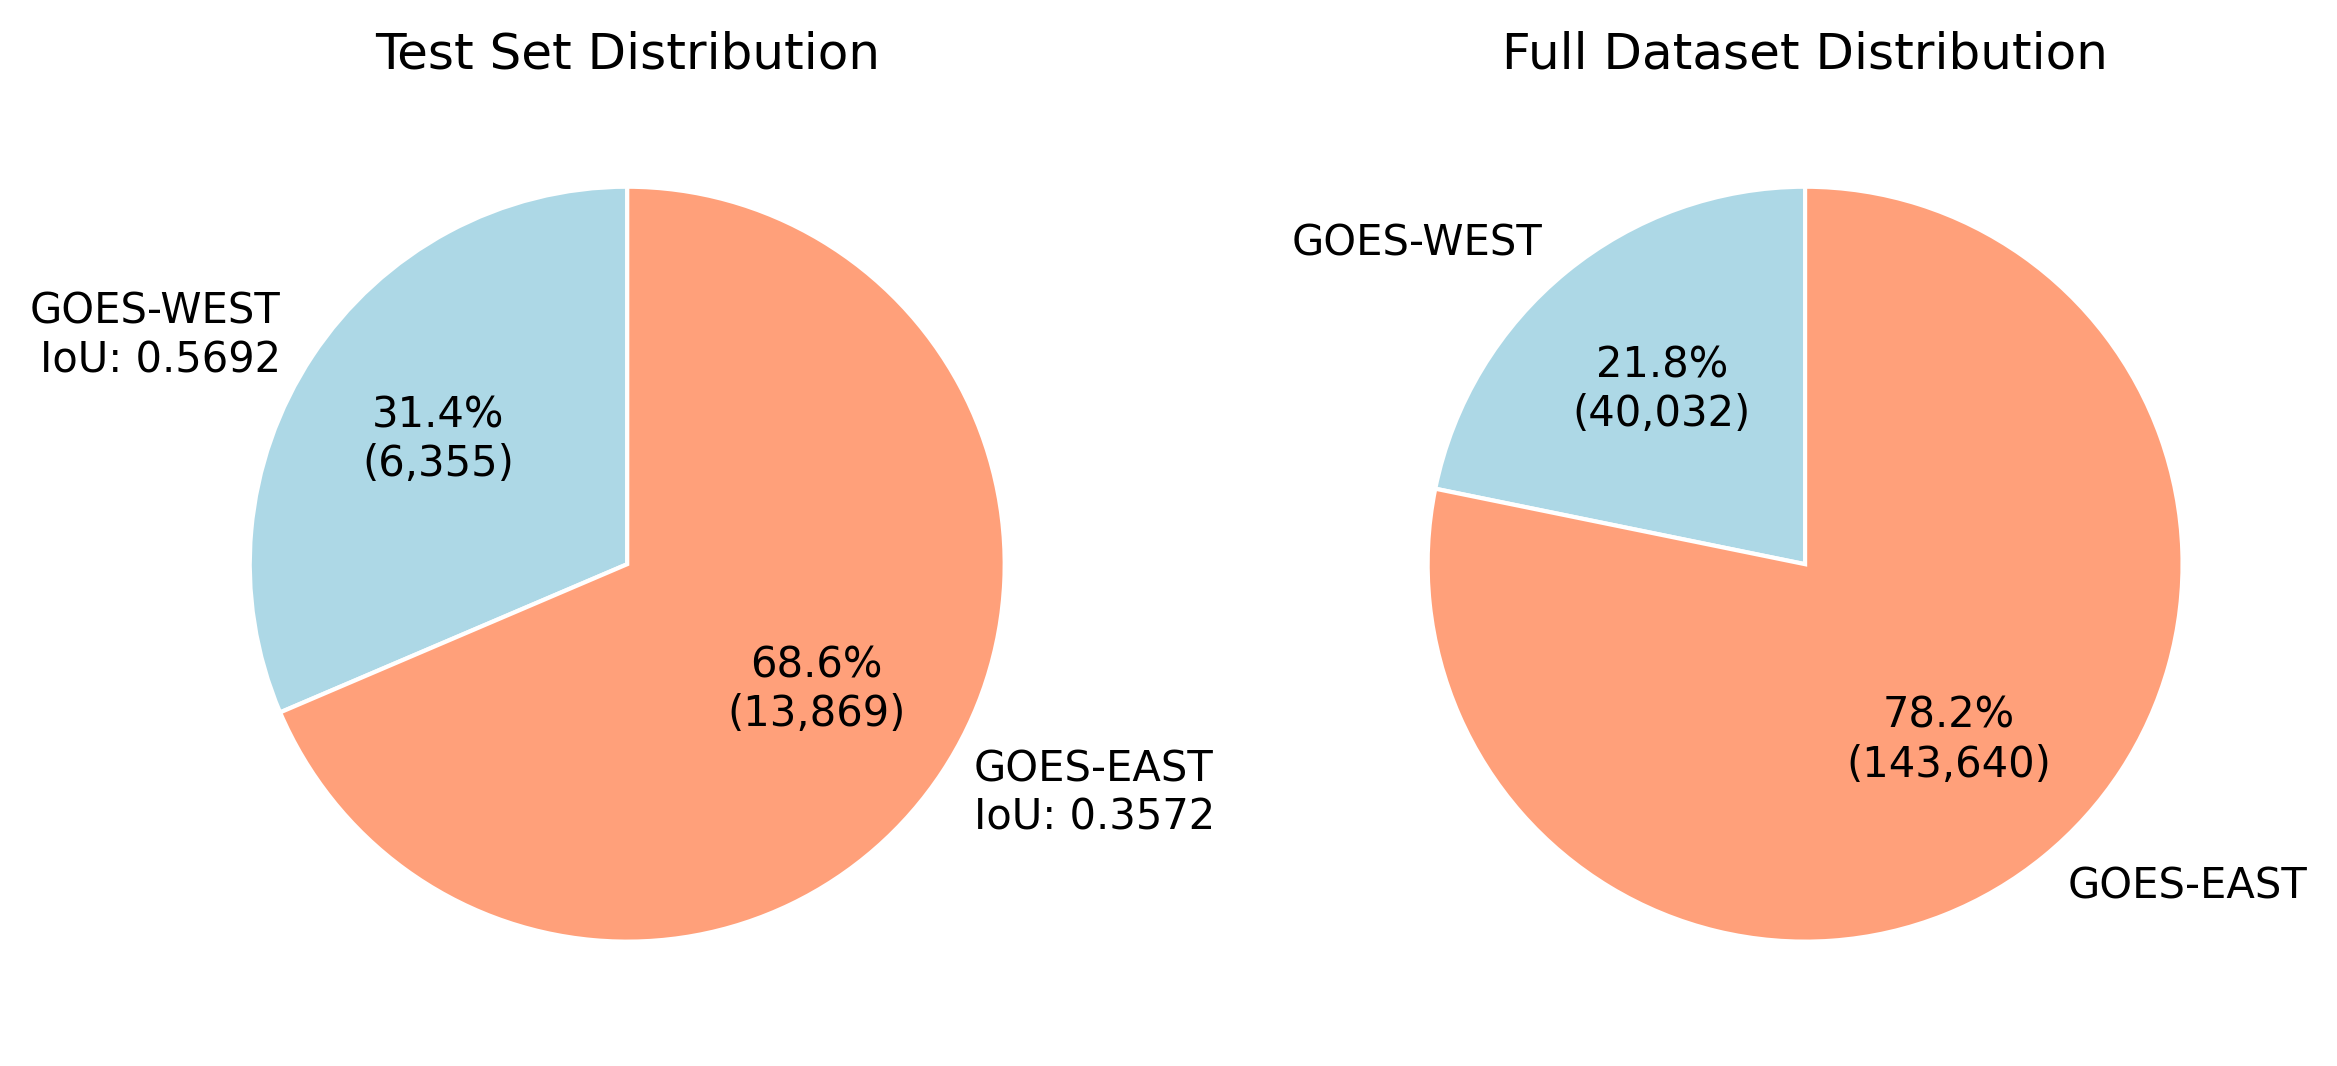
\includegraphics[width=\linewidth]{stat_figs/satellite_test_full_dataset.png}
    \caption{The SmokeViz test set (left) and full SmokeViz dataset (right) distributions by observational satellite.}
    \label{sat_dataset}
\end{figure}

\subsection{Sunset/Sunrise Bias}

As mentioned in the limitations, there may have been a bias introduced towards correctly classifying imagery close to sunrise or sunset. This bias may not only be introduced by our Mie-derived dataset that was used to train \(f_{\circ}\), but also in the original HMS annotations. The configuration of the sun, smoke and satellite give the highest signal-to-noise ratio at the times near the sunrise and sunset, making smoke more easily observable by analysts. In contrast, the diurnal variations of wildfires cause the fire radiative power to be highest around solar noon \cite{diurnal}. Table \ref{two_hr_iou} shows how the IoU between \(f_c\) predictions and analyst annotations for the test data from either \(\mathcal{D}_M\) or \(\mathcal{D}_p\) vary based on proximity to sunset/sunrise. One explanation for better values for midday samples could be due to higher amounts of fire activity midday and higher amounts of atmospheric interaction noise early/late in the day. Another difference we see from table \ref{two_hr_iou} is the split of closer to daylight boundaries is shifted towards midday between \(\mathcal{D}_M\) to \(\mathcal{D}_p\). This is because, for \(\mathcal{D}_p\), we are choosing the imagery with the best overlap to the analyst product rather than the image from \(\mathcal{D}_M\) that optimized for highest possible signal-to-noise ratio if given constant signal.

\begin{figure}[!htb]
    \centering
    \includegraphics[width=\linewidth]{stat_figs/Mie_vs_PL_midday.png}
    \caption{Mie Derived dataset vs SmokeViz test sets with IoU}
    \label{DM_vs_DP}
\end{figure}

\begin{figure}[!htb]
    \centering
        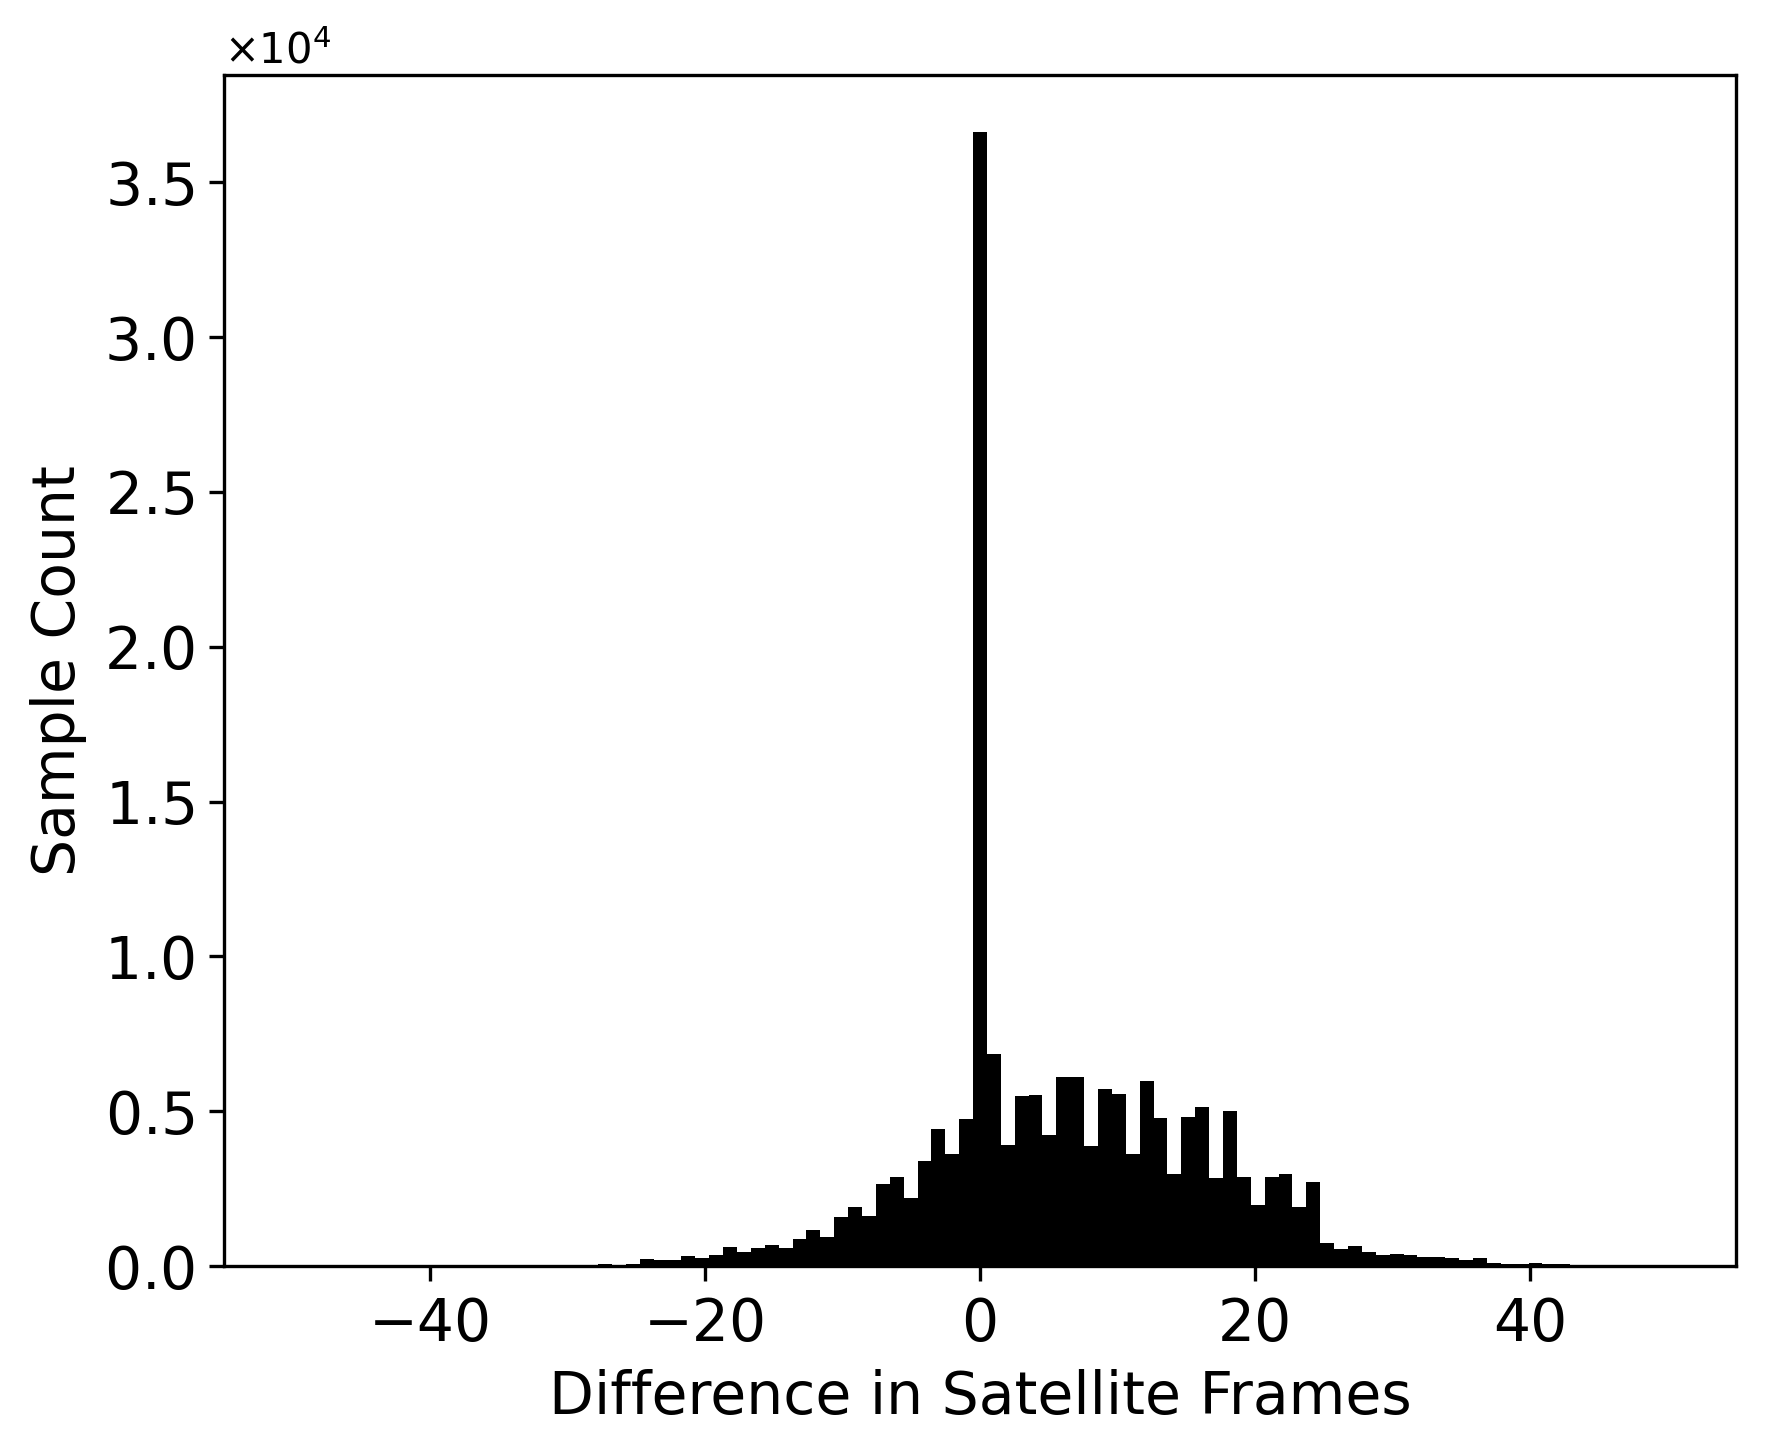
\includegraphics[width=0.49\textwidth]{stat_figs/sample_count_vs_diff_frames.png}
        \caption{The number of satellite frame difference between the \(\mathcal{D}_M\) satellite image and \(\mathcal{D}_p\) chosen satellite image. GOES Full disk images are generated on 10 minute intervals. The number of samples that use the same satellite image in both datasets was 36,608 (\(\approx\)20\%).}
        \label{frame_diff}
\end{figure}



\subsection{Qualitative Analysis on Performance}

Figure \ref{poor} gives some examples of when SmokeViz does not perform well in comparison to the HMS analyst annotations. In the first column example, SmokeViz confuses a smoke-like cloud for smoke, something it generally tends to not seem to have issues with, but this is an counter example to that trend. The second through last columns all miss distinctive plumes that should be classified as either medium or heavy density smoke. In contrast, we show what SmokeViz looks like when it performs well in comparison to the HMS smoke product in figure \ref{good}.

\begin{figure}[!htb]
    \centering
    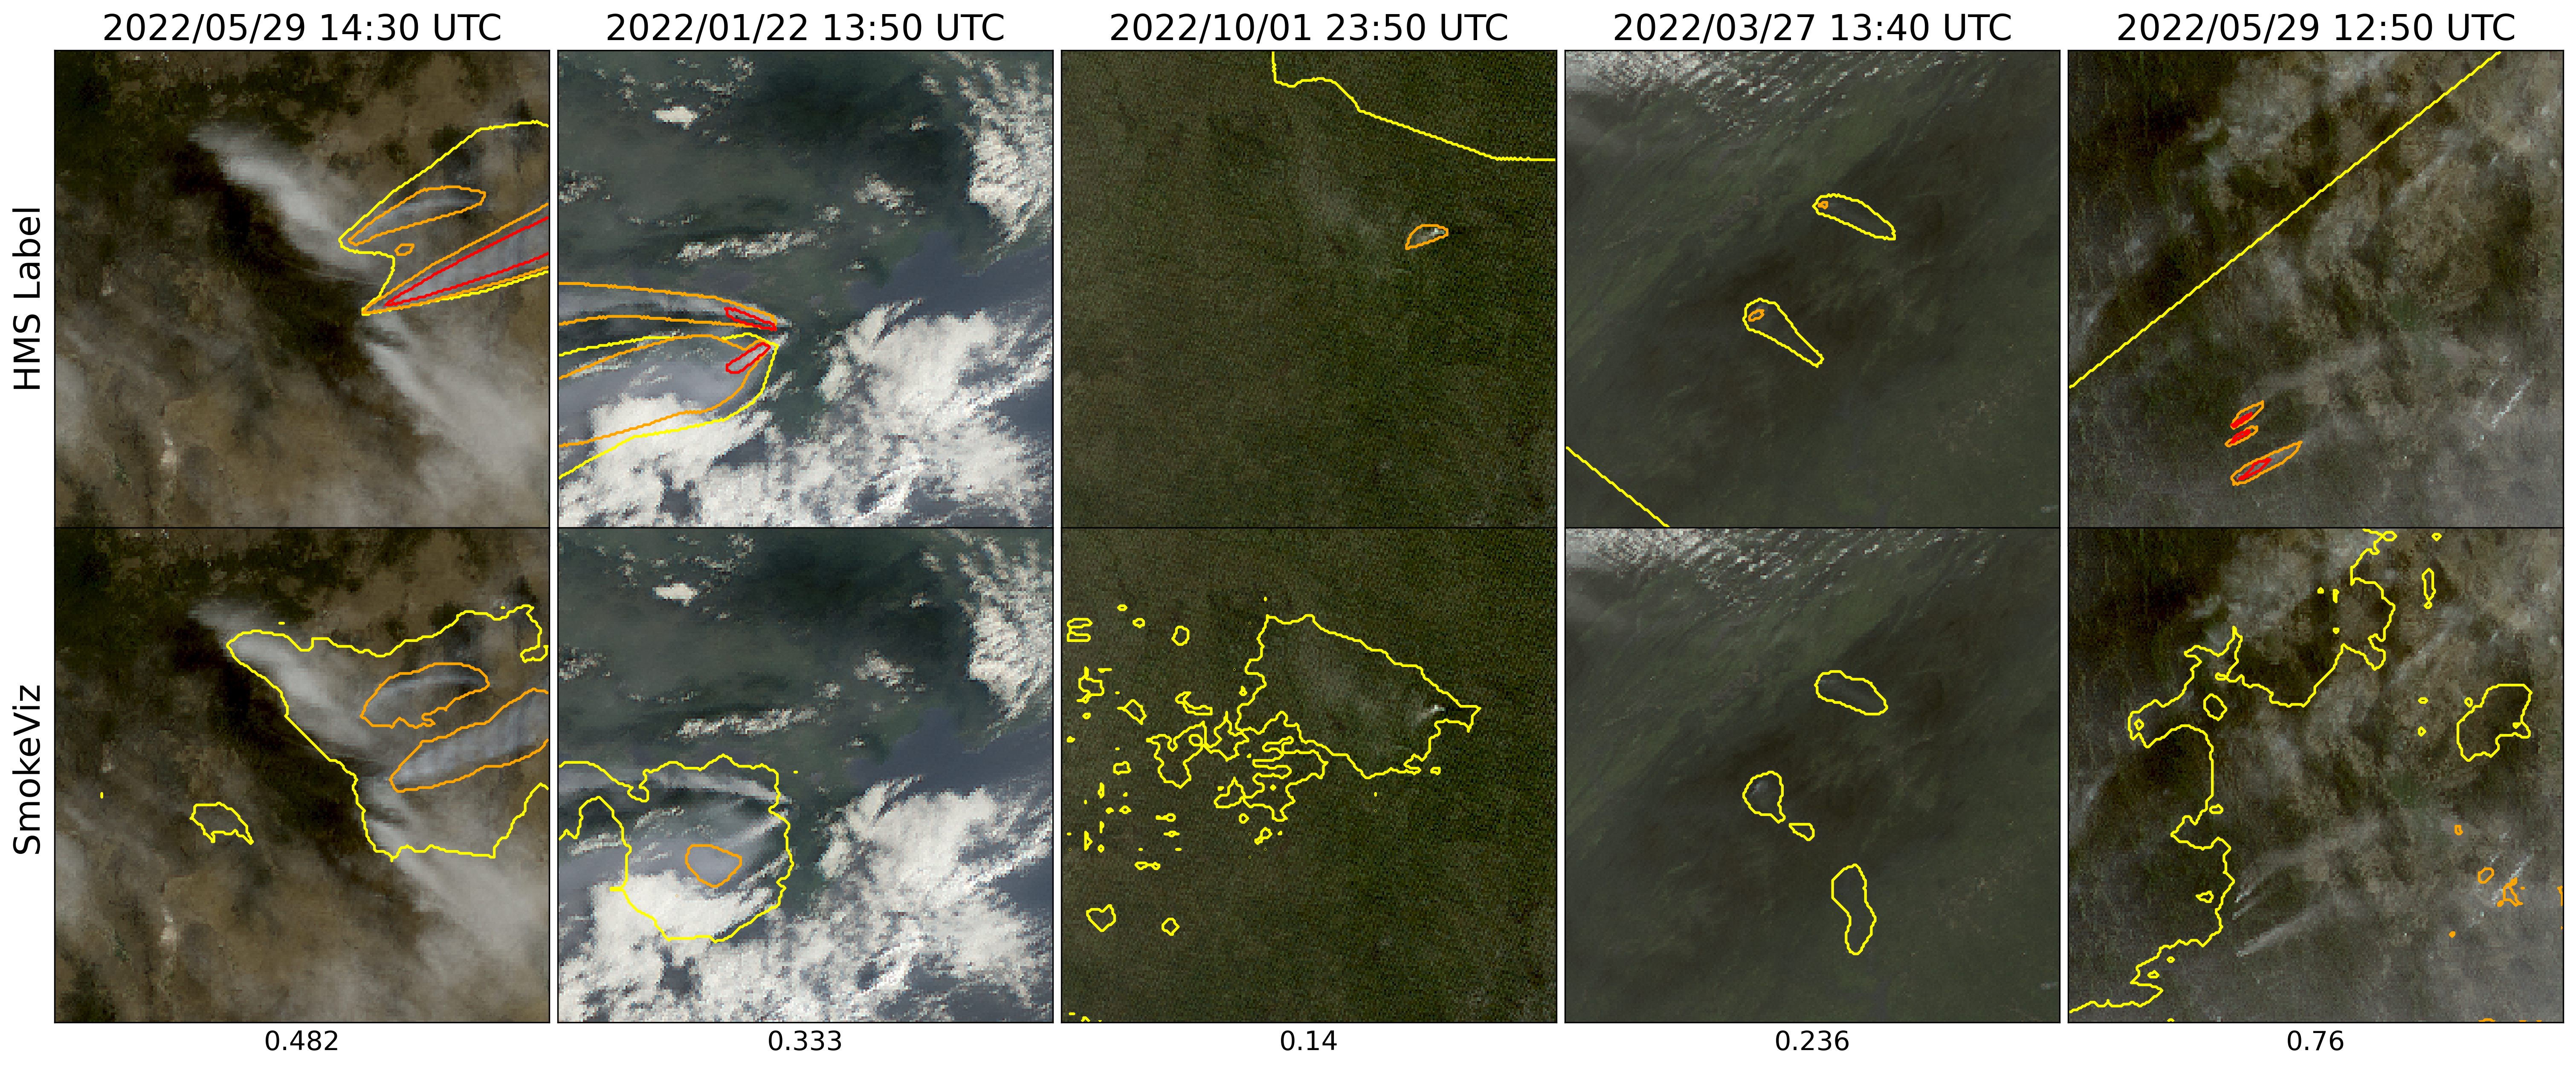
\includegraphics[width=\linewidth]{stat_figs/bad_results.png}
    \caption{Examples of Smoke Viz performing poorly.}
    \label{poor}
\end{figure}


\begin{figure}[!htb]
    \centering
    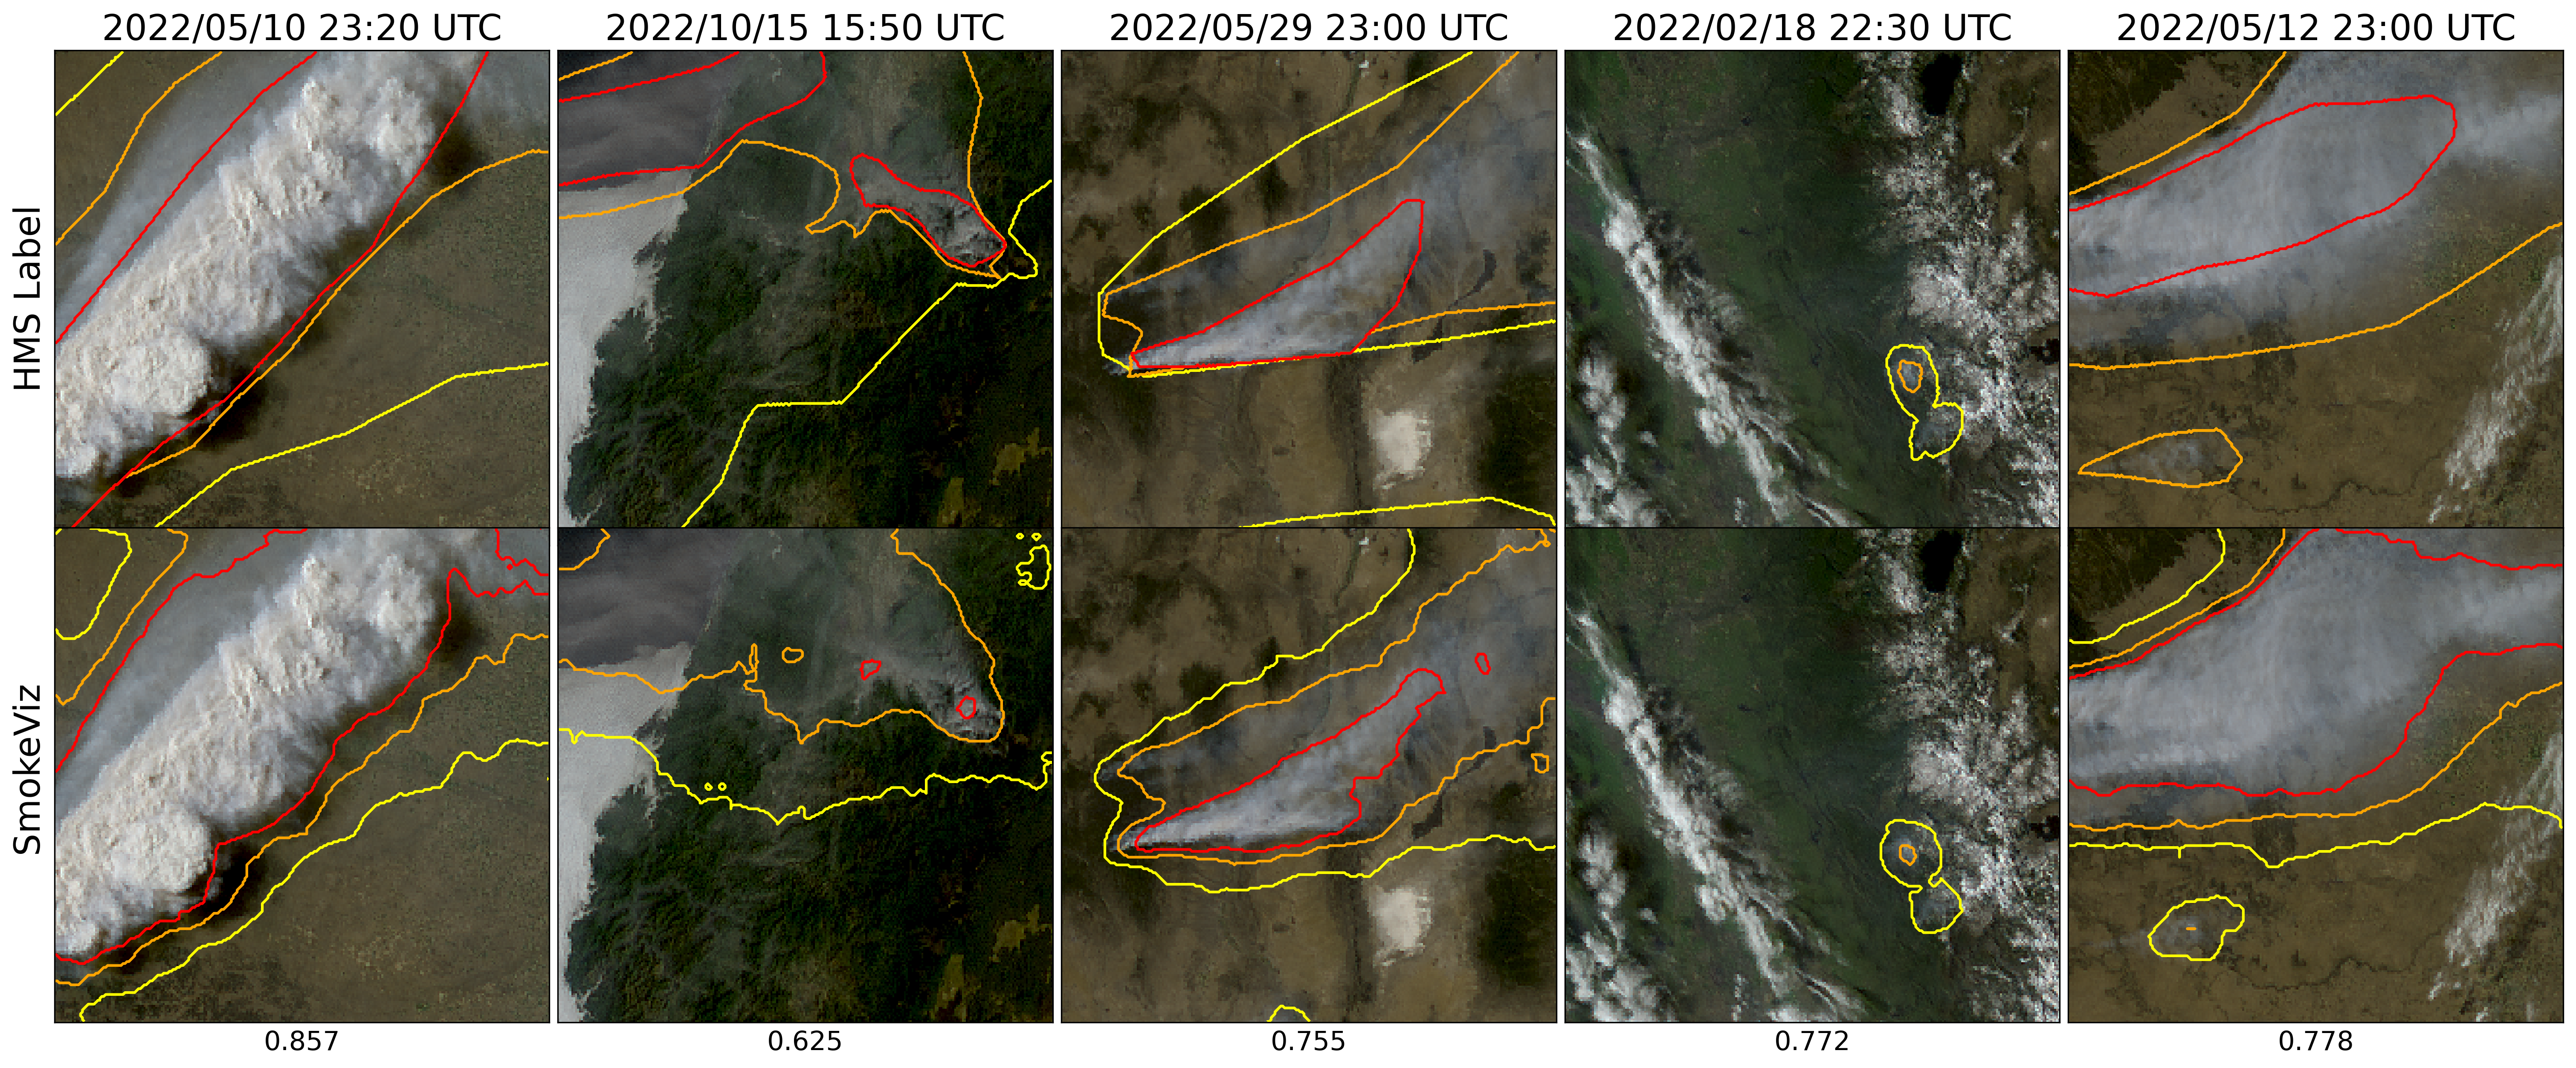
\includegraphics[width=\linewidth]{stat_figs/good_results.png}
    \caption{Examples of Smoke Viz performing well.}
    \label{good}
\end{figure}


\subsection{Machine Learning Reproducibility}

All relevant code is accessible at \url{https://github.com/anonymous-smokeviz/SmokeViz}. The models presented in this paper are not optimized for performance, but are intended to create sufficient pseudo-labels to develop the SmokeViz dataset and then compare the performance of SmokeViz against the original dataset. The child model used in the PLDR process was chosen by running the models shown in table \ref{child} on the Mie-derived dataset and choosing the model with the highest IoU. The hyperparameters used in for the models are shown in table \ref{hyper}. We use the Adam optimizer that will adapt the learning rate during training and is suited for problems with large amounts of data. Batch size was chosen due to the necessity to run the model on limited resources. 

\begin{table}[!htb] 
    \caption{Comparison of segmentation model IoU metrics on the Mie-Derived dataset. Based on the IoU results, the first column that uses EfficientNet and PSPNet was used as for \(f_{\circ}\).}\label{child}
    \centering
    \begin{tabular}{lccccc}
        \toprule
        \textbf{encoder} & EfficientNet\cite{efficientnetv2} & \cite{efficientnetv2} & EfficientViT\cite{efficientvit} & \cite{efficientvit}& ViT \cite{vit} \\
        \textbf{decoder} &  PSPNet\cite{pspnet} & DeepLabV3+\cite{deeplab} & Segformer\cite{segformer} & UperNet \cite{upernet}& DPT\cite{dpt} \\
        \midrule
        Heavy   &	\textbf{0.3221}	& 0.2893	&	0.2185	&	0.3099	&	0.2466 \\
        Medium  &	\textbf{0.4288}	& 0.4091	&	0.3977	&   0.4041	&	0.3135 \\
        Light   &	\textbf{0.5044}	& 0.4424	&	0.4331	&	0.4274	&	0.4964 \\
        Overall &	\textbf{0.4677}	& 0.4172	&   0.4054	&	0.4098	&	0.4331 \\
        \bottomrule
    \end{tabular}
\end{table}

\begin{table}
    \caption{Hyperparameters used to create \(f_{\circ}\) and \(f_{c}\).}
  \label{hyper}
  \centering
  \begin{tabular}{ll}
    \toprule
    parameter & value \\ 
    \midrule
    epochs & 100 \\
    learning rate & 1e-4 \\
    batch size & 16 \\
    optimizer & Adam \\
    \bottomrule
  \end{tabular}
\end{table}


\bibliography{references}
\end{document}
\pagebreak

